\section{Math 202a - HW4 - Dan Davison - \texttt{ddavison@berkeley.edu}}

% 1. 10/10 3. 10/10 5. 10/10 6. 10/10

\begin{mdframed}
  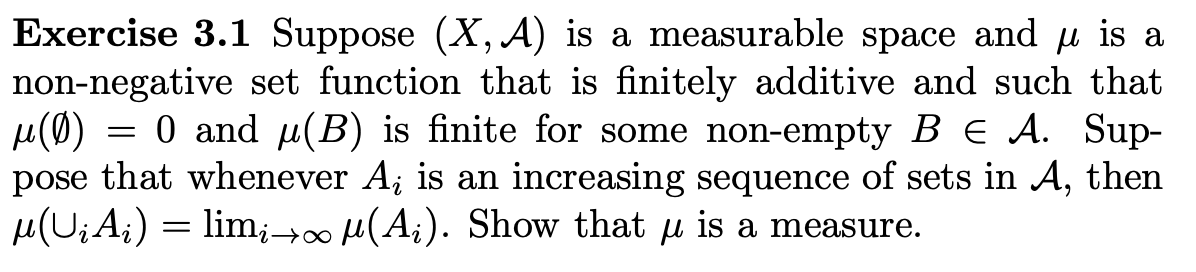
\includegraphics[width=400pt]{img/analysis--berkeley-202a-hw04-f604.png}
\end{mdframed}
\begin{claim*}
  $\mu$ is a measure.
\end{claim*}
\begin{proof}~\\
  It is given that $\mu$ is non-negative and that $\mu(\emptyset) = 0$. We must prove that $\mu$ is countably
  additive.

  So let $B_1, B_2, \dots$ be a pairwise disjoint countable collection of subsets of $X$. We want to show
  that $\mu(\bigcup_{i=1}^\infty B_i) = \sum_{i=1}^\infty \mu(B_i)$.

  Define $A_j = \bigcup_{i \leq j} B_i$ for $j=1, 2, \ldots$, so that $A_1, A_2, \ldots$ is an increasing
  sequence of sets. Note that $\bigcup_{i=1}^\infty B_i = \bigcup_{j=1}^\infty A_j$ therefore, by
  hypothesis,
  $\mu\big(\bigcup_{i=1}^\infty B_i\big) = \mu\big(\bigcup_{j=1}^\infty A_j\big) = \lim_{j\to\infty} \mu(A_j)$.

  Now, from finite additivity we have
  \begin{align*}
    \mu(A_j) = \mu(\bigcup_{i \leq j} B_i) = \sum_{i\leq j} \mu(B_i),
  \end{align*}
  therefore
  \begin{align*}
    \mu\big(\bigcup_{i=1}^\infty B_i\big) = \lim_{j\to\infty} \sum_{i\leq j} \mu(B_i) = \sum_{i=1}^\infty \mu(B_i),
  \end{align*}
  as required.
\end{proof}

\newpage
\begin{mdframed}
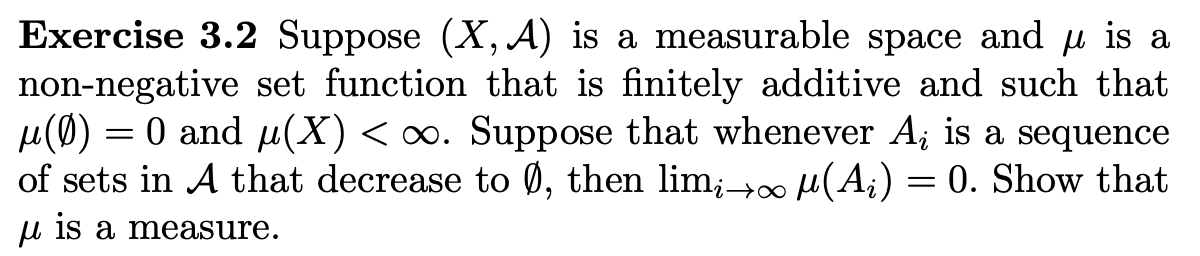
\includegraphics[width=400pt]{img/analysis--berkeley-202a-hw04-c187.png}
\end{mdframed}

\begin{proof}~\\
  It is given that $\mu$ is non-negative and that $\mu(\emptyset) = 0$. In order to prove that $\mu$ is a
  measure, we must prove that $\mu$ is countably additive.

  Let $B_1, B_2, \ldots \in \mc A$ be a countable pairwise disjoint collection of sets. It is given that $\mu$
  is finitely additive, so we have
  \begin{align*}
    \sum_{i=1}^\infty \mu(B_i) = \lim_{n\to\infty} \sum_{i=1}^n \mu(B_i) = \lim_{n\to\infty} \mu(\bigcup_{i=1}^n B_i).
  \end{align*}
  Therefore in order to prove countable additivity, it suffices to prove
  \begin{align*}
    \mu\big(\bigcup_{i=1}^\infty B_i \big) = \lim_{n\to\infty} \mu(\bigcup_{i=1}^n B_i).
  \end{align*}
  Let $Y = \bigcup_{i=1}^\infty B_i$ and define $S_n := \bigcup_{i=1}^n B_i$, so that the result we want to
  prove is now
  \begin{align*}
    \mu(Y) = \lim_{n\to\infty} \mu(S_n).
  \end{align*}
  Note that the sequence $(Y \setminus S_1), (Y \setminus S_2), \ldots$ decreases to $\emptyset$,
  therefore $\lim_{n\to\infty}\mu(Y \setminus S_n) = 0$. Note also that by finite additivity of $\mu$ we have,
  for all $n \in \N$,
  \begin{align*}
    \mu(Y) = \mu(S_n) + \mu(Y \setminus S_n).
  \end{align*}
  Taking the limit as $n \to \infty$ we have
  \begin{align*}
    \mu(Y) = \lim_{n\to\infty} \mu(S_n),
  \end{align*}
  as required.
\end{proof}


\newpage
\begin{mdframed}
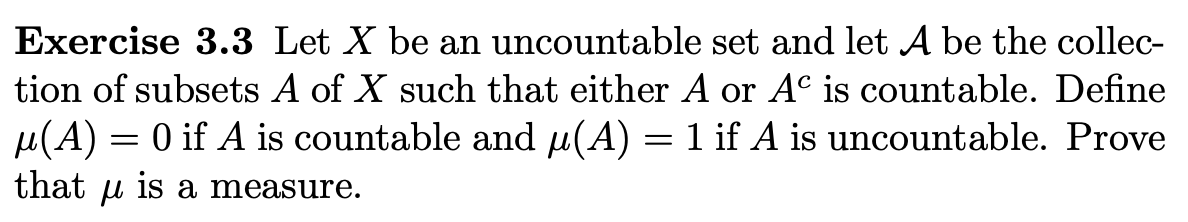
\includegraphics[width=400pt]{img/analysis--berkeley-202a-hw04-b168.png}
\end{mdframed}
\begin{proof}~\\
  $\emptyset$ is countable, therefore we have $\mu(\emptyset) = 0$ as required, and it remains to show
  that $\mu$ is countably additive.

  So let $B_1, B_2, \ldots$ be a pairwise disjoint countable collection of subsets of $X$. We want to show
  that $\mu(\bigcup_{i=1}^\infty B_i) = \sum_{i=1}^\infty \mu(B_i)$.

  % Consider $\bigcup_{i=1}^\infty B_i$. It could be uncountable, since the $B_i$ could be a countable partition
  % of the entire set $X$. Could it also be countable? Yes, since the $B_i$ could be singletons. So we must
  % handle both cases.

  First suppose $\bigcup_{i=1}^\infty B_i$ is countable. Then no $B_i$ is uncountable. Therefore $\mu(B_i) = 0$
  for all $i$ and we have
  \begin{align*}
    \sum_{i=1}^\infty \mu(B_i) = \sum_{i=1}^\infty 0 = 0 = \mu\big(\bigcup_{i=1}^\infty B_i\big),
  \end{align*}
  as required.

  Next, suppose $\bigcup_{i=1}^\infty B_i$ is uncountable. We want to show
  that $\sum_{i=1}^\infty \mu(B_i) = 1$. Equivalently, we want to show that exactly one of the $B_i$ is
  uncountable.

  Note that we have by hypothesis that either $B_i$ is countable or $B_i^c$ is countable, for all $i$. Clearly
  some $B_i$ is uncountable or else we would
  have $\sum_{i=1}^\infty \mu(B_i) = \sum_{i=1}^\infty 0 = 0 \neq \mu\big(\bigcup_{i=1}^\infty B_i\big)$.

  Suppose for a contradiction that there exists $j \neq k$ such that $B_j$ and $B_k$ are uncountable. Note
  that $B_j$ and $B_k$ are disjoint, therefore $B_k \subseteq B_j^c$. But $B_j^c$ is countable, therefore $B_k$
  is countable; a contradiction. Therefore no such pair $j, k$ exists and we conclude that exactly one of
  the $B_i$ is uncountable, as required.
\end{proof}

\newpage
\begin{mdframed}
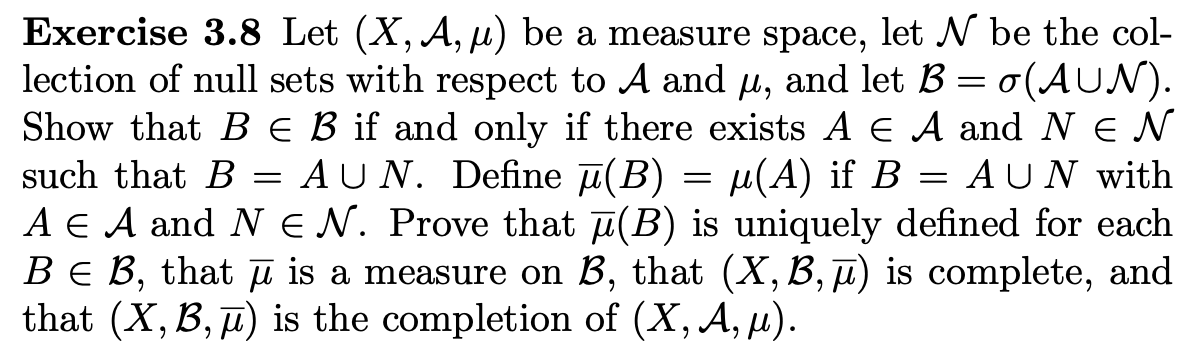
\includegraphics[width=400pt]{img/analysis--berkeley-202a-hw04-c88b.png}
\end{mdframed}

\begin{claim*}\label{claim-3-8-1}
  $B \in \mc B$ if and only if there exists $A \in \mc A$ and $N \in \mc N$ such that $B = A \cup N$.
\end{claim*}

\begin{proof}~\\
  Define $\mc B = \sigma(\mc A \cup \mc N)$ and let $\mc C$ be the collection of sets of the specified form,
  i.e. $\mc C = \{A \cup N ~:~ A \in \mc A, N \in \mc N\}$. We want to show that $\mc B = \mc C$.

  To show that $\mc C \subseteq \mc B$, let $A \in \mc A$ and $N \in \mc N$. Then $A \in \mc A \cup \mc N$,
  therefore $A \in \sigma(\mc A \cup \mc N) =: \mc B$. Similarly $N \in \mc A \cup \mc N$,
  therefore $N \in \sigma(\mc A \cup \mc N) =: \mc B$.

  Let $C = A \cup N$ be an arbitrary element of $\mc C$. Since $\mc B$ is a $\sigma$-algebra and $A \in \mc B$
  and $N \in \mc B$, we have $C \in \mc B$. Therefore $\mc C \subseteq \mc B$.

  To show that $\mc B \subseteq \mc C$, first note that $\emptyset \in \mc N$,
  therefore $\mc A = \{ A \cup \emptyset ~:~ A \in \mc A \} \subseteq \mc C$. Similarly $\emptyset \in \mc A$
  implies that $\mc N \subset \mc C$. Therefore $\mc A \cup \mc N \subset \mc C$.

  Next we will show that $\mc C$ is a $\sigma$-algebra. Since $\mc A \cup \mc N \subset \mc C$, it will then
  follow that $\mc B := \sigma(\mc A \cup \mc N) \subseteq \sigma(\mc C) = \mc C$ as required.

  Since $\emptyset \in \mc A$ and $\emptyset \in \mc N$, we have $\emptyset \in \mc C$.

  Let $A \in \mc A$ and $N \in \mc N$. Then $(A \cup N)^C = A^c \cap N^c$. Since $A^c \in \mc A$
  and $N^c \in \mc N$, we see that $(A \cup N)^C \in \mc C$ and thus that $\mc C$ is closed under complements.

  It remains to show that $\mc C$ is closed under countable unions of pairwise disjoint collections. So
  let $A_1, A_2, \ldots \in \mc A$ be pairwise disjoint and let $N_1, N_2, \ldots \in \mc N$ be pairwise
  disjoint, and define $C_i = A_i \cup N_i$ for all $i$. Then
  \begin{align*}
    \bigcup_{i=1}^\infty C_i
    &= \bigcup_{i=1}^\infty \big(A_i \cup N_i\big) \\
    &= \lim_{n\to\infty} \bigcup_{i=1}^n \big(A_i \cup N_i\big) \\
    &= \lim_{n\to\infty} \big(\bigcup_{i=1}^n A_i\big) \bigcup \big(\bigcup_{i=1}^n N_i \big) \\
    &= \big(\bigcup_{i=1}^\infty A_i\big) \bigcup \big(\bigcup_{i=1}^\infty N_i \big).
  \end{align*}
  Since $\big(\bigcup_{i=1}^\infty A_i\big) \in \mc A$ and $\big(\bigcup_{i=1}^\infty N_i\big) \in \mc N$ we see that $\big(\bigcup_{i=1}^\infty C_i\big) \in C$ as required.
\end{proof}


\begin{lemma}[A measure is finitely sub-additive]\label{lemma-3-8-subadditivity}
  Let $\mc A$ be a $\sigma$-algebra, let $A_1, A_2 \subseteq \mc A$ and let $\mu$ be a measure on $\mc A$.
  Then $\mu(A_1 \cup A_2) \leq \mu(A_1) + \mu(A_2)$.
\end{lemma}

\begin{proof}~\\
  Note that $A_1, (A_2 \setminus A_1), \emptyset, \emptyset, \ldots$ is a countable pairwise disjoint
  collection with union equal to $A_1 \cup A_2$. Therefore, using countable additivity followed by
  monotonicity,
  \begin{align*}
    \mu(A_1 \cup A_2)
    &= \mu(A_1) + \mu(A_2 \setminus A_1) + 0 + \cdots \\
    &\leq \mu(A_1) + \mu(A_2).
  \end{align*}
\end{proof}

\begin{claim*}
  Define $\bar{\mu}(B) = \mu(A)$ if $B = A \cup N$ with $A \in \mc A$ and $N \in \mc N$.

  Then $\bar{\mu}(B)$ is uniquely defined for each $B \in \mc B$.
\end{claim*}

\begin{proof}~\\
  Let $B \in \mc B$. We will show that $\bar\mu(B)$ is the same for all decompositions of the
  form $B = A \cup N$ where $A \in \mc A$ and $N \in \mc N$.

  So let $A, A' \in \mc A$ and $N, N' \in \mc N$ be such that $A \cup N = A' \cup N' = B$.

  We must show that $\bar{\mu}(A \cup N) = \bar{\mu}(A' \cup N')$. This is equivalent to showing
  that $\mu(A) = \mu(A')$.

  Note that, since $N'$ is a null set, there exists $A_{N'} \in \mc A$ with $N' \subseteq A_{N'}$
  and $\mu(A_{N'}) = 0$. Therefore we have
  \begin{align*}
    A
    &\subseteq A' \cup N' \\
    &\subseteq A' \cup A_{N'}.
  \end{align*}
  By monotonicity of $\mu$ we have $\mu(A) \leq \mu(A' \cup A_{N'})$. And by finite sub-additivity of $\mu$
  (see lemma \eqref{lemma-3-8-subadditivity}) we have
  \begin{align*}
    \mu(A)
    &\leq \mu(A') + \mu(\cup A_{N'}) \\
    &= \mu(A') + 0 \\
    &= \mu(A').
  \end{align*}
  Similarly, since $N$ is a null set, there exists $A_{N} \in \mc A$ with $N \subseteq A_{N}$
  and $\mu(A_{N}) = 0$, and by an equivalent argument to the above (switch the primes on $A$ and $A'$, and
  remove the prime from $N'$) we have $\mu(A') \leq \mu(A)$.

  Therefore $\mu(A) = \mu(A')$ as required.
\end{proof}

\begin{claim*}
  $\bar{\mu}$ is a measure on $\mc B$.
\end{claim*}

\begin{proof}~\\
  Since $\emptyset \in \mc A$ and $\emptyset \in \mc N$ we
  have $\bar\mu(\emptyset) = \bar\mu(\emptyset \cup \emptyset) = \mu(\emptyset) = 0$ as required. It remains to
  show that $\bar\mu$ is countably additive on $\mc B$.

  So let $B_1, B_2, \ldots \in \mc B$ be countable and pairwise disjoint, where for each $i$ these decompose
  as $B_i = A_i \cup N_i$ with $A_i \in \mc A$ and $N_i \in \mc N$. Then
  \begin{align*}
    \bigcup_{i=1}^\infty B_i
    &= \lim_{n\to\infty}\bigcup_{i=1}^n (A_i \cup N_i) \\
    &= \lim_{n\to\infty} \Big(\bigcup_{i=1}^n A_i ~\cup~ \bigcup_{i=1}^n N_i\Big) \\
    &= \bigcup_{i=1}^\infty A_i ~\cup~ \bigcup_{i=1}^\infty N_i.
  \end{align*}
  Note that $\bigcup_{i=1}^\infty A_i \in \mc A$, since $\mc A$ is a $\sigma$-algebra.

  Note also that, since the $B_i$ are pairwise disjoint, so the $A_i$ are pairwise disjoint and also the $N_i$
  are pairwise disjoint.

  Using pairwise disjointness of the $N_i$ we see that $\bigcup_{i=1}^\infty N_i \in \mc N$, since
  \begin{align*}
    \mu\Big(\bigcup_{i=1}^\infty N_i\Big) = \sum_{i=1}^\infty \mu(N_i) = \sum_{i=1}^\infty 0 = 0.
  \end{align*}
  Thus we see that
  \begin{align*}
    \bar\mu\Big(\bigcup_{i=1}^\infty A_i ~\cup~ \bigcup_{i=1}^\infty N_i\Big) = \mu\Big(\bigcup_{i=1}^\infty A_i\Big),
  \end{align*}
  since the set on the left is of the form $A \cup N$ with $A \in \mc A$ and $N \in \mc N$.

  Therefore, using pairwise disjointness of the $A_i$ and countable additivity of $\mu$, we have
  \begin{align*}
    \bar\mu\Big(\bigcup_{i=1}^\infty B_i\Big)
    = \mu\Big(\bigcup_{i=1}^\infty A_i\Big)
    = \sum_{i=1}^\infty \mu(A_i)
    = \sum_{i=1}^\infty \bar\mu(B_i),
  \end{align*}
  as required.
\end{proof}

\begin{claim*}
  $(X, \mc B, \bar{\mu})$ is complete.
\end{claim*}

\begin{proof}~\\
  By definition, $(X, \mc B, \bar{\mu})$ is complete if all null sets with respect to $\bar\mu$ and $\mc B$ are
  in $\mc B$.

  Let $N_1$ be a null set with respect to $\bar\mu$ and $\mc B$. Then there exists $B_1 \in \mc B$
  with $\bar\mu(B_1) = 0$ such that $N_1 \subseteq B_1$.

  Since $B_1 \in \mc B$ it is of the form $B_1 = A_1 \cup N_2$ where $A_1 \in \mc A$ and $N_2 \in \mc N$. Therefore
  $N_1 \subseteq A_1 \cup N_2$.

  Furthermore, since $N_2 \in \mc N$, there exists $A_2 \in \mc A$ such that $N_2 \subseteq A_2$.
  Therefore $N_1 \subseteq A_1 \cup A_2$.

  But then $N_1 \in \mc N$, hence $N_1 \in \mc B := \sigma(\mc A \cup \mc N)$ as required.
\end{proof}

\begin{claim*}
  $(X, \mc B, \bar{\mu})$ is the completion of $(X, \mc A, \mu)$.
\end{claim*}

\begin{proof}~\\
  We've already shown that $(X, \mc B, \bar\mu)$ is complete, with $\mc A \subseteq \mc B$ and with $\bar{\mu}$
  an extension of $\mu$. It remains to show that no smaller $\sigma$-algebra exists that satisfies those same
  conditions.

  So let $(X, \mc B', \mu')$ be complete, with $\mc A \subseteq \mc B$ and with $\mu'$ an extension of $\mu$.
  We will show that $\mc B \subseteq \mc B'$.

  Let $A \cup N \in \mc B$, where $A \in \mc A$ and $N \in \mc N$. We know that $N \in \mc B'$, since $\mc B'$
  is complete. And we know that $A \in \mc B'$, since $A \in \mc A \subseteq \mc B'$.
  Therefore $A \cup N \in \mc B'$, since $\mc B'$ is closed under finite unions.

  Therefore $\mc B \subseteq \mc B'$, as required.
\end{proof}

\newpage
\begin{mdframed}
  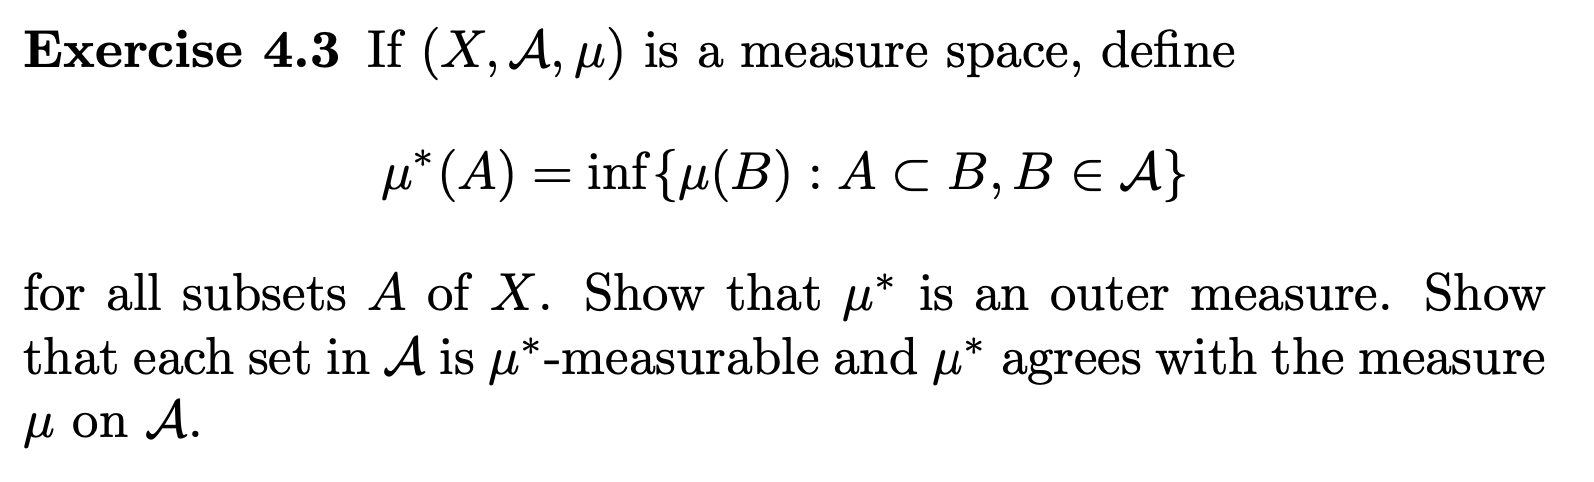
\includegraphics[width=400pt]{img/analysis--berkeley-202a-hw-0d98.png}
\end{mdframed}

\begin{claim*}
  $\mu^*$ is an outer measure.
\end{claim*}

\begin{proof}~\\
  Note that $\mu^*(\emptyset) = 0$, since $\emptyset$ is covered by $\emptyset \in \mc A$ with $\mu(\emptyset) = 0$.

  It remains to show that $\mu^*$ is countably sub-additive.

  Let $A_1, A_2, \ldots \in X$. We must show that
  \begin{align*}
    \mu^*\Big(\bigcup_{i=1}^\infty A_i\Big) \leq \sum_{i=1}^\infty \mu^*(A_i).
  \end{align*}
  Note that $X \in \mc A$, therefore every $A_i$ is a subset of some set in $\mc A$.

  Let $\epsilon > 0$. For $i \in \N$, let $C_i \in \mc A$ be such that $A_i \subseteq C_{i}$ with
  \begin{align*}
    \mu(C_{i}) < \mu^*(A_i) + \epsilon/2^i.
  \end{align*}
  (We can do this because $\mu^*(A_i)$ is defined as an infimum over covering sets; if for some $\epsilon_i$
  there did not exist a $C_i$ such that $\mu(C_{i}) < \mu^*(A_i) + \epsilon_i$ then $\mu^*(A_i) + \epsilon_i$
  would be a lower bound; a contradiction.)

  Then we have
  \begin{align*}
    \mu^*\Big(\bigcup_{i=1}^\infty A_i\Big) \leq \sum_{i=1}^\infty \mu(C_{i}) < \sum_{i=1}^\infty \mu^*(A_i) + \epsilon.
  \end{align*}
  Since $\eps > 0$ is arbitrary, this implies
  \begin{align*}
    \mu^*\Big(\bigcup_{i=1}^\infty A_i\Big) \leq \sum_{i=1}^\infty \mu^*(A_i),
  \end{align*}
  as required.
\end{proof}

\begin{claim*}
  Each set in $\mc A$ is $\mu^*$-measurable.
\end{claim*}

\begin{proof}~\\
  Let $B \in \mc A$. We must show that
  \begin{align*}
    \mu^*(B) = \mu^*(B \cap E) + \mu^*(B \cap E^c),
  \end{align*}
  for every $E \subseteq X$.

  So let $E \subseteq X$. Note that
  \begin{align*}
    \mu^*(B) \leq \mu^*(B \cap E) + \mu^*(B \cap E^c).
  \end{align*}
  is a statement of finite sub-additivity of $\mu^*$, which follows from countable sub-additivity of $\mu^*$
  (form a countable sequence with $B_1 = B \cap E$, $B_2 = B \cap E^c$, and $B_i = \emptyset$ for $i > 2$ and
  apply countable additivity), so what remains to prove is that
  \begin{align*}
    \mu^*(B) \geq \mu^*(B \cap E) + \mu^*(B \cap E^c).
  \end{align*}
  Let $\eps > 0$ and let $C \in \mc A$ be such that $B \subseteq C$ with
  \begin{align*}
    \mu(C_i) < \mu^*(B) + \eps.
  \end{align*}
  (As before, to see that we can do this note that if we could not, then $\mu^*(B) + \eps$ would be a lower
  bound, contradicting $\mu^*(B)$ as the infimum.)

  Then
  \begin{align*}
    \mu^*(B) + \eps
    &> \mu(C) \\
    &= \mu(C \cap E) + \mu(C \cap E^c) \\
    &\geq \mu^*(B \cap E) + \mu^*(B \cap E^c).
  \end{align*}
  Since $\eps$ is arbitrary it follows that
  \begin{align*}
    \mu^*(B) \geq \mu^*(B \cap E) + \mu^*(B \cap E^c),
  \end{align*}
  as required.
\end{proof}


\begin{claim*}
  $\mu^*$ agrees with the measure $\mu$ on $\mc A$.
\end{claim*}

\begin{proof}~\\
  Let $B \in \mc A$ and let $\mc B = \{B' : B \subseteq B', B' \in \mc A\}$. We must show
  that $\mu^*(B) = \mu(B)$. We have
  \begin{align*}
    \mu^*(B)
    &:= \inf \{\mu(B') : B' \in \mc B\} \\
    &=  \inf \{\mu(B \cup (B' \setminus B)) : B' \in \mc B\} \\
    &=  \inf \{\mu(B) + \mu(B' \setminus B) : B' \in \mc B\}.
  \end{align*}
  Let $M = \{\mu(B) + \mu(B' \setminus B) : B' \in \mc B\}$; the set over which this last infimum is taken.
  Note that $B \in \mc B$, therefore $\mu(B) = \mu(B) + \mu(\emptyset) \in M$. Furthermore, since $\mu$ is
  non-negative, $m \geq \mu(B)$ for all $m \in M$. Therefore $\mu(B)$ is a minimum of $M$, and therefore it is
  the infimum of $M$, as required.
\end{proof}

\newpage
\begin{mdframed}
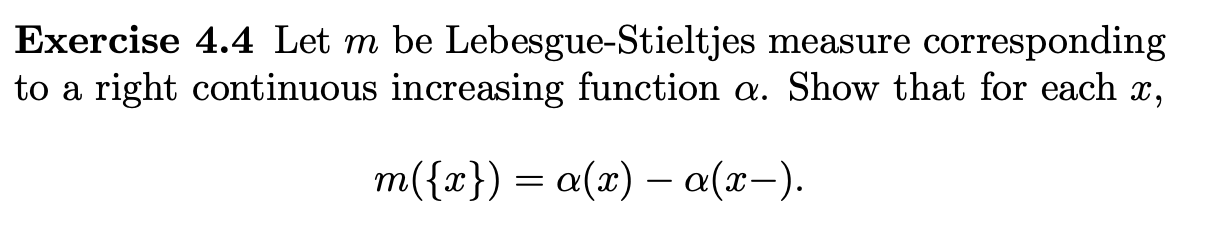
\includegraphics[width=400pt]{img/analysis--berkeley-202a-hw04-c0b6.png}
\end{mdframed}

\begin{proof}~\\
  Let $\alpha: \R \to \R$ be right-continuous and increasing, and let $m$ be Lebesgue-Stieltjes measure. By
  definition,
  \begin{align*}
    m(\{x\}) := \inf \Big\{\sum_{i=1}^\infty \ell(I_i) : \{x\} \subseteq \bigcup_{i=1}^\infty I_i, ~ I_i \subseteq \R \text{~for all~}i\Big\}.
  \end{align*}
  Recall that for any measure $\mu$, given a sequence of sets $A_i \downarrow A$, we
  have $\lim_{n\to\infty} \mu(A_i) = \mu(A)$. Therefore we have
  \begin{align*}
    m\big(\{x\}\big)
    &= \lim_{n\to\infty} m\big((x - 1/n, x]\big) \\
    &= \lim_{n\to\infty} \alpha(x) - \alpha(x - 1/n) \\
    &= \alpha(x) - \lim_{n\to\infty} \alpha(x - 1/n) \\
    &= \alpha(x) - \alpha(x-).
  \end{align*}
\end{proof}




\begin{comment}
\newpage
  EXERCISE 3.3 FROM OLD VERSION
  \begin{mdframed}
    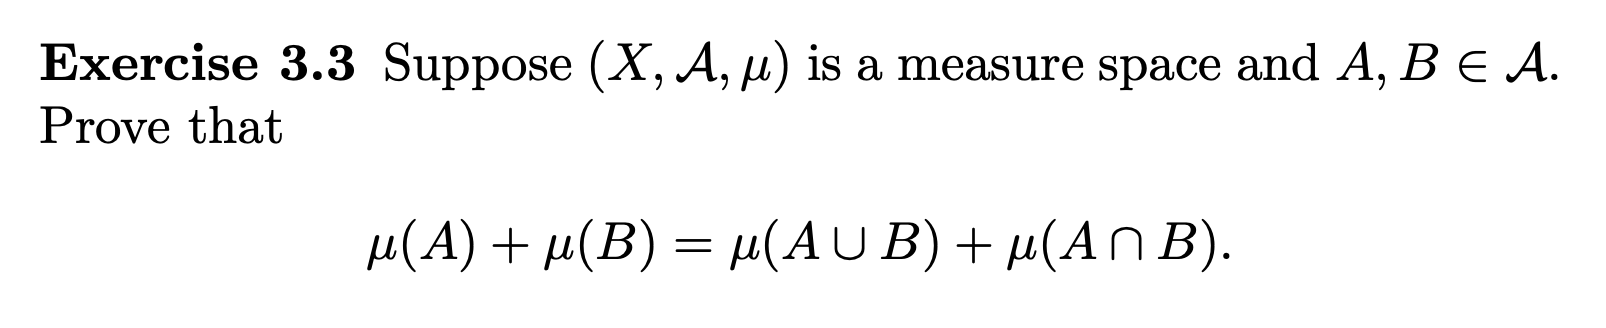
\includegraphics[width=400pt]{img/analysis--berkeley-202a-hw-2389.png}
  \end{mdframed}

  \begin{proof}~\\
    From finite additivity we have
    \begin{align*}
      \mu(A \cup B) &= \mu(A) + \mu(A \setminus B). \\
      \mu(A \cup B) &= \mu(B) + \mu(B \setminus A).
    \end{align*}
    Summing these gives
    \begin{align*}
      2\mu(A \cup B)
      = \mu(A) + \mu(B) + \mu(A \triangle B)
    \end{align*}
    But $\{A \triangle B, A \cap B\}$ is a partition of $A \cup B$ hence from finite additivity
    again $\mu(A \triangle B) + \mu(A \cap B) = \mu(A \cup B)$. Therefore
    \begin{align*}
      2\mu(A \cup B) = \mu(A) + \mu(B) + \mu(A \cup B) - \mu(A \cap B),
    \end{align*}
    or equivalently
    \begin{align*}
      \mu(A \cup B) = \mu(A) + \mu(B) - \mu(A \cap B).
    \end{align*}
  \end{proof}

  \begin{mdframed}
    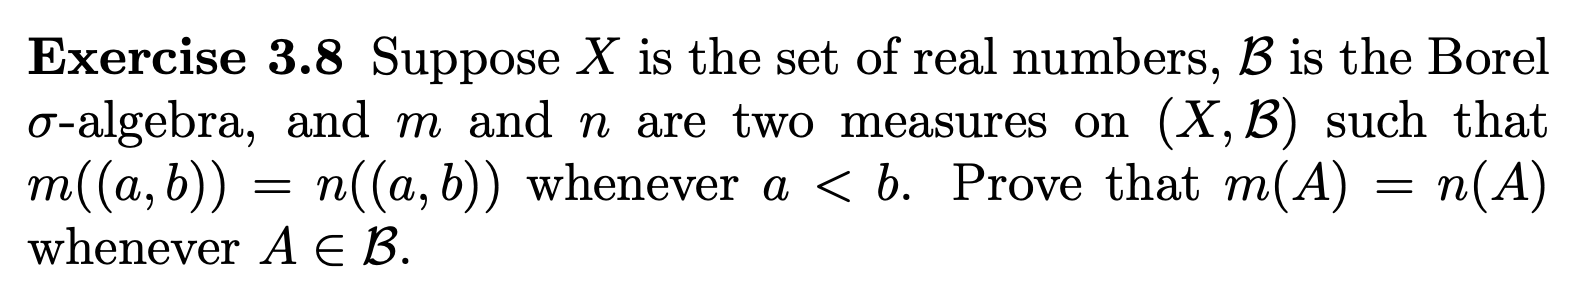
\includegraphics[width=400pt]{img/analysis--berkeley-202a-hw-3a79.png}
  \end{mdframed}

  \begin{claim*}
    If $m$ and $n$ have the same value on any open interval in $B$ then they have the same value on any set
    in $\mc B$.
  \end{claim*}

  \begin{proof}~\\
    Let $\mc O$ be the collection of open subsets of $\R$.

    Let $O \in \mc O$. Then $O$ can be written as a countable union of disjoint open intervals, $O = \bigcup_i I_i$. Therefore
    \begin{align*}
      m(O) = m(\bigcup_i I_i) = \sum_i m(I_i) = \sum_i n(I_i) = n(O).
    \end{align*}
    By definition, $\mc B = \sigma(\mc O)$. We want to show that measures $m$ and $n$ agree on every set $A \in \mc B$.

    Let $A \in \mc B$ and suppose $m(A) = n(A)$. Then
    \begin{align*}
      m(A^c) = m(X) - m(A) = n(X) - n(A) = n(A^c).
    \end{align*}
  \end{proof}
\end{comment}
